\documentclass{standalone}
\usepackage{tikz}
\usetikzlibrary{patterns, positioning}


\begin{document}
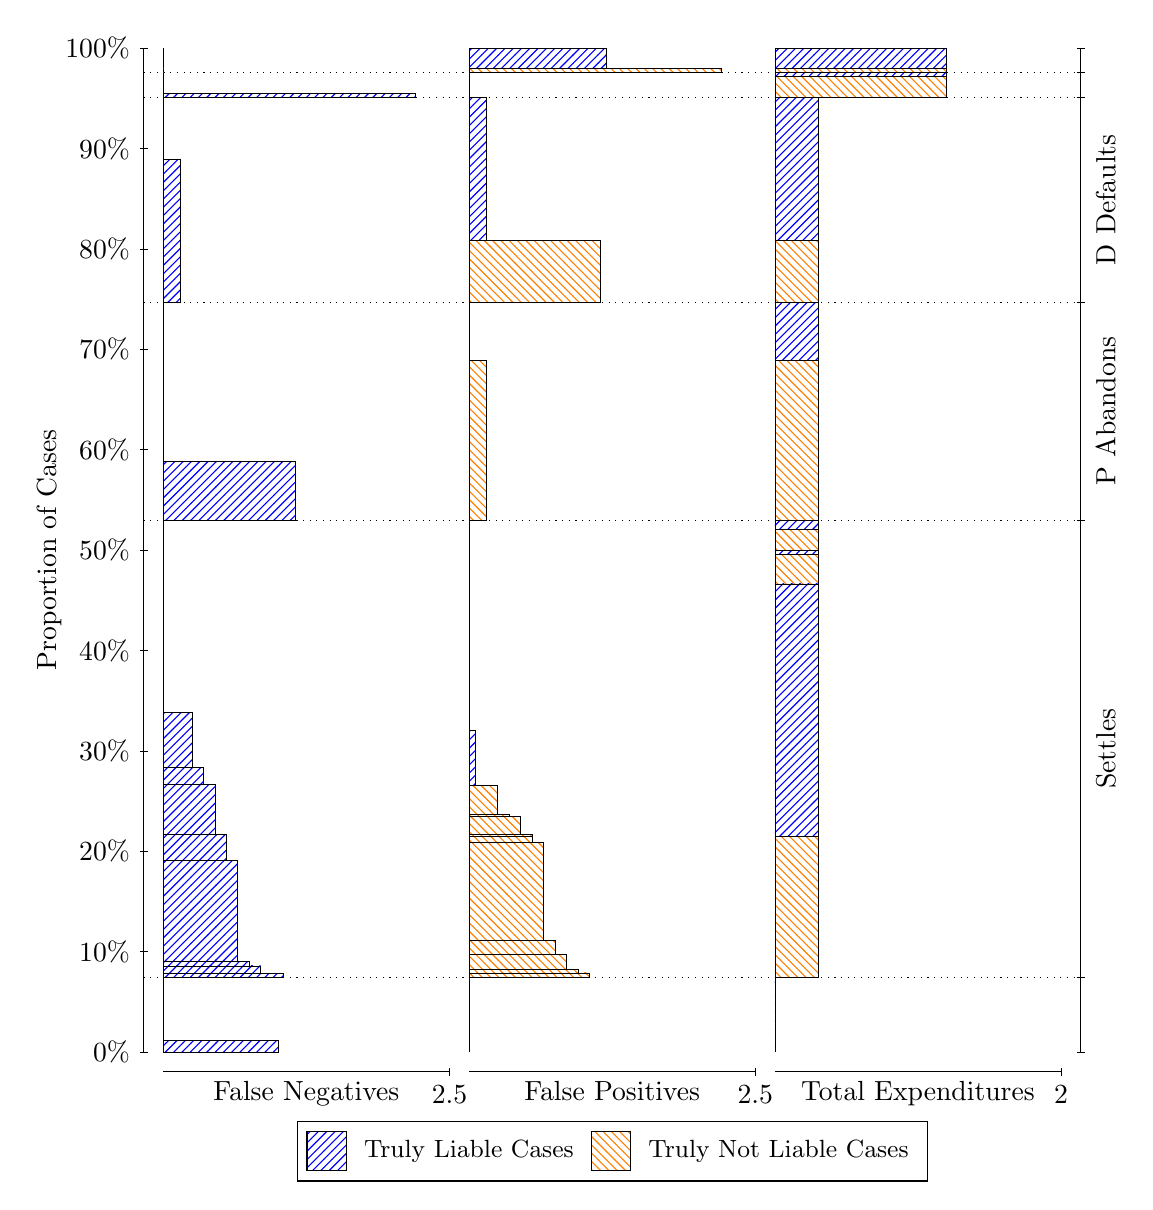
\begin{tikzpicture}
\draw[black, very thin] (1.5,1.75) -- (1.5,14.5);
\node[rotate=90, text=black, anchor=center] at (0.3, 8.125) {Proportion of Cases};
\draw[black, very thin] (1.45,1.75) -- (1.55,1.75);
\node[text=black, anchor=east] at (1.45, 1.75) {0\%};
\draw[black, very thin] (1.45,3.025) -- (1.55,3.025);
\node[text=black, anchor=east] at (1.45, 3.025) {10\%};
\draw[black, very thin] (1.45,4.3) -- (1.55,4.3);
\node[text=black, anchor=east] at (1.45, 4.3) {20\%};
\draw[black, very thin] (1.45,5.575) -- (1.55,5.575);
\node[text=black, anchor=east] at (1.45, 5.575) {30\%};
\draw[black, very thin] (1.45,6.85) -- (1.55,6.85);
\node[text=black, anchor=east] at (1.45, 6.85) {40\%};
\draw[black, very thin] (1.45,8.125) -- (1.55,8.125);
\node[text=black, anchor=east] at (1.45, 8.125) {50\%};
\draw[black, very thin] (1.45,9.4) -- (1.55,9.4);
\node[text=black, anchor=east] at (1.45, 9.4) {60\%};
\draw[black, very thin] (1.45,10.675) -- (1.55,10.675);
\node[text=black, anchor=east] at (1.45, 10.675) {70\%};
\draw[black, very thin] (1.45,11.95) -- (1.55,11.95);
\node[text=black, anchor=east] at (1.45, 11.95) {80\%};
\draw[black, very thin] (1.45,13.225) -- (1.55,13.225);
\node[text=black, anchor=east] at (1.45, 13.225) {90\%};
\draw[black, very thin] (1.45,14.5) -- (1.55,14.5);
\node[text=black, anchor=east] at (1.45, 14.5) {100\%};

\draw[black, very thin] (13.4,1.75) -- (13.4,14.5);
\draw[black, very thin] (13.35,1.75) -- (13.45,1.75);
\node[anchor=west] at (13.35, 1.75) {};
\draw[black, very thin] (13.35,2.6967) -- (13.45,2.6967);
\node[anchor=west] at (13.35, 2.6967) {};
\draw[black, very thin] (13.35,8.5039) -- (13.45,8.5039);
\node[anchor=west] at (13.35, 8.5039) {};
\draw[black, very thin] (13.35,11.273) -- (13.45,11.273);
\node[anchor=west] at (13.35, 11.273) {};
\draw[black, very thin] (13.35,13.871) -- (13.45,13.871);
\node[anchor=west] at (13.35, 13.871) {};
\draw[black, very thin] (13.35,14.191) -- (13.45,14.191);
\node[anchor=west] at (13.35, 14.191) {};
\draw[black, very thin] (13.35,14.5) -- (13.45,14.5);
\node[anchor=west] at (13.35, 14.5) {};

\draw[black, very thin, pattern color=blue, pattern=north east lines] (1.75,1.75) rectangle (3.2033,1.894);
\draw[black, very thin, pattern color=orange, pattern=north west lines] (1.75,1.894) rectangle (1.75,2.6967);
\draw[black, very thin, pattern color=blue, pattern=north east lines] (1.75,2.6967) rectangle (3.276,2.747);
\draw[black, very thin, pattern color=blue, pattern=north east lines] (1.75,2.747) rectangle (3.1307,2.7526);
\draw[black, very thin, pattern color=blue, pattern=north east lines] (1.75,2.7526) rectangle (2.9853,2.8433);
\draw[black, very thin, pattern color=blue, pattern=north east lines] (1.75,2.8433) rectangle (2.84,2.9036);
\draw[black, very thin, pattern color=blue, pattern=north east lines] (1.75,2.9036) rectangle (2.6947,4.1875);
\draw[black, very thin, pattern color=blue, pattern=north east lines] (1.75,4.1875) rectangle (2.5493,4.5169);
\draw[black, very thin, pattern color=blue, pattern=north east lines] (1.75,4.5169) rectangle (2.404,5.1503);
\draw[black, very thin, pattern color=blue, pattern=north east lines] (1.75,5.1503) rectangle (2.2587,5.3672);
\draw[black, very thin, pattern color=blue, pattern=north east lines] (1.75,5.3672) rectangle (2.1133,6.0653);
\draw[black, very thin, pattern color=orange, pattern=north west lines] (1.75,6.0653) rectangle (1.75,8.5039);
\draw[black, very thin, pattern color=blue, pattern=north east lines] (1.75,8.5039) rectangle (3.4213,9.247);
\draw[black, very thin, pattern color=orange, pattern=north west lines] (1.75,9.247) rectangle (1.75,11.273);
\draw[black, very thin, pattern color=blue, pattern=north east lines] (1.75,11.273) rectangle (1.968,13.083);
\draw[black, very thin, pattern color=orange, pattern=north west lines] (1.75,13.083) rectangle (1.75,13.871);
\draw[black, very thin, pattern color=blue, pattern=north east lines] (1.75,13.871) rectangle (4.9473,13.92);
\draw[black, very thin, pattern color=orange, pattern=north west lines] (1.75,13.92) rectangle (1.75,14.191);
\draw[black, very thin, pattern color=orange, pattern=north west lines] (1.75,14.191) rectangle (1.75,14.24);
\draw[black, very thin, pattern color=blue, pattern=north east lines] (1.75,14.24) rectangle (1.75,14.5);
\draw[black, very thin, pattern color=orange, pattern=north west lines] (5.6333,1.75) rectangle (5.6333,2.5527);
\draw[black, very thin, pattern color=blue, pattern=north east lines] (5.6333,2.5527) rectangle (5.6333,2.6967);
\draw[black, very thin, pattern color=orange, pattern=north west lines] (5.6333,2.6967) rectangle (7.1593,2.7558);
\draw[black, very thin, pattern color=orange, pattern=north west lines] (5.6333,2.7558) rectangle (7.014,2.8024);
\draw[black, very thin, pattern color=orange, pattern=north west lines] (5.6333,2.8024) rectangle (6.8687,2.9905);
\draw[black, very thin, pattern color=orange, pattern=north west lines] (5.6333,2.9905) rectangle (6.7233,3.1686);
\draw[black, very thin, pattern color=orange, pattern=north west lines] (5.6333,3.1686) rectangle (6.578,4.409);
\draw[black, very thin, pattern color=orange, pattern=north west lines] (5.6333,4.409) rectangle (6.4327,4.4904);
\draw[black, very thin, pattern color=orange, pattern=north west lines] (5.6333,4.4904) rectangle (6.4327,4.5155);
\draw[black, very thin, pattern color=orange, pattern=north west lines] (5.6333,4.5155) rectangle (6.2873,4.743);
\draw[black, very thin, pattern color=orange, pattern=north west lines] (5.6333,4.743) rectangle (6.142,4.7634);
\draw[black, very thin, pattern color=orange, pattern=north west lines] (5.6333,4.7634) rectangle (5.9967,5.1352);
\draw[black, very thin, pattern color=blue, pattern=north east lines] (5.6333,5.1352) rectangle (5.706,5.8334);
\draw[black, very thin, pattern color=blue, pattern=north east lines] (5.6333,5.8334) rectangle (5.6333,8.5039);
\draw[black, very thin, pattern color=orange, pattern=north west lines] (5.6333,8.5039) rectangle (5.8513,10.53);
\draw[black, very thin, pattern color=blue, pattern=north east lines] (5.6333,10.53) rectangle (5.6333,11.273);
\draw[black, very thin, pattern color=orange, pattern=north west lines] (5.6333,11.273) rectangle (7.3047,12.061);
\draw[black, very thin, pattern color=blue, pattern=north east lines] (5.6333,12.061) rectangle (5.8513,13.871);
\draw[black, very thin, pattern color=orange, pattern=north west lines] (5.6333,13.871) rectangle (5.6333,14.142);
\draw[black, very thin, pattern color=blue, pattern=north east lines] (5.6333,14.142) rectangle (5.6333,14.191);
\draw[black, very thin, pattern color=orange, pattern=north west lines] (5.6333,14.191) rectangle (8.8307,14.24);
\draw[black, very thin, pattern color=blue, pattern=north east lines] (5.6333,14.24) rectangle (7.3773,14.5);
\draw[black, very thin, pattern color=orange, pattern=north west lines] (9.5167,1.75) rectangle (9.5167,2.5527);
\draw[black, very thin, pattern color=blue, pattern=north east lines] (9.5167,2.5527) rectangle (9.5167,2.6967);
\draw[black, very thin, pattern color=orange, pattern=north west lines] (9.5167,2.6967) rectangle (10.062,4.4904);
\draw[black, very thin, pattern color=blue, pattern=north east lines] (9.5167,4.4904) rectangle (10.062,7.6943);
\draw[black, very thin, pattern color=orange, pattern=north west lines] (9.5167,7.6943) rectangle (10.062,8.0662);
\draw[black, very thin, pattern color=blue, pattern=north east lines] (9.5167,8.0662) rectangle (10.062,8.1166);
\draw[black, very thin, pattern color=orange, pattern=north west lines] (9.5167,8.1166) rectangle (10.062,8.3895);
\draw[black, very thin, pattern color=blue, pattern=north east lines] (9.5167,8.3895) rectangle (10.062,8.5039);
\draw[black, very thin, pattern color=orange, pattern=north west lines] (9.5167,8.5039) rectangle (10.062,10.53);
\draw[black, very thin, pattern color=blue, pattern=north east lines] (9.5167,10.53) rectangle (10.062,11.273);
\draw[black, very thin, pattern color=orange, pattern=north west lines] (9.5167,11.273) rectangle (10.062,12.061);
\draw[black, very thin, pattern color=blue, pattern=north east lines] (9.5167,12.061) rectangle (10.062,13.871);
\draw[black, very thin, pattern color=orange, pattern=north west lines] (9.5167,13.871) rectangle (11.697,14.142);
\draw[black, very thin, pattern color=blue, pattern=north east lines] (9.5167,14.142) rectangle (11.697,14.191);
\draw[black, very thin, pattern color=orange, pattern=north west lines] (9.5167,14.191) rectangle (11.697,14.24);
\draw[black, very thin, pattern color=blue, pattern=north east lines] (9.5167,14.24) rectangle (11.697,14.5);
\draw[black, dotted] (1.5,2.6967) -- (13.4,2.6967);
\draw[black, dotted] (1.5,8.5039) -- (13.4,8.5039);
\draw[black, dotted] (1.5,11.273) -- (13.4,11.273);
\draw[black, dotted] (1.5,13.871) -- (13.4,13.871);
\draw[black, dotted] (1.5,14.191) -- (13.4,14.191);
\draw[black, very thin] (1.75,1.5) -- (5.3833,1.5);
\node[text=black, anchor=north] at (3.5667, 1.5) {False Negatives};
\draw[black, very thin] (5.3833,1.45) -- (5.3833,1.55);
\node[text=black, anchor=north] at (5.3833, 1.45) {2.5};

\draw[black, very thin] (5.6333,1.5) -- (9.2667,1.5);
\node[text=black, anchor=north] at (7.45, 1.5) {False Positives};
\draw[black, very thin] (9.2667,1.45) -- (9.2667,1.55);
\node[text=black, anchor=north] at (9.2667, 1.45) {2.5};

\draw[black, very thin] (9.5167,1.5) -- (13.15,1.5);
\node[text=black, anchor=north] at (11.333, 1.5) {Total Expenditures};
\draw[black, very thin] (13.15,1.45) -- (13.15,1.55);
\node[text=black, anchor=north] at (13.15, 1.45) {2};


\node[text=black, centered, rotate=90] at (13.72, 5.6003) {Settles};
\node[text=black, centered, rotate=90] at (13.72, 9.8885) {P Abandons};
\node[text=black, centered, rotate=90] at (13.72, 12.572) {D Defaults};



\draw (7.449999999999999,1.5) node[draw=none] (baseCoordinate) {};
\begin{scope}[align=center]
        \matrix[scale=0.5, draw=black, below=0.5cm of baseCoordinate, nodes={draw}, column sep=0.1cm]{
            \node[rectangle, draw, minimum width=0.5cm, minimum height=0.5cm, pattern color=blue, pattern=north east lines] {}; &
            \node[draw=none, font=\small, text=black] (B) {Truly Liable Cases}; &
            \node[rectangle, draw, minimum width=0.5cm, minimum height=0.5cm, pattern color=orange, pattern=north west lines] {}; &
            \node[draw=none, font=\small, text=black] (B) {Truly Not Liable Cases}; \\
            };
\end{scope}

\end{tikzpicture}
\end{document}